\documentclass{cys}
\usepackage[ansinew]{inputenc}

\usepackage{graphicx}
\usepackage{tikz}
\usetikzlibrary{automata,positioning,fit}



\title{Theoretical and Experimental Approach to SMP Scheduling}

\author{Jnaneshwar Weibel}

% \affil{ 
% University of British Columbia, \authorcr
% Country             
% \authorcr \authorcr
% author1@xxx.xx
% \authorcr  \authorcr
% }

\begin{document}

\maketitle

\begin{abstract}
Over the years computer hardware has grown increasingly efficient; in particular, the capability for multiprocessing allows systems to distribute work across multiple CPUs.  Modern operating systems and their respective schedulers have the opportunity to make policy decisions about this distribution that may influence the performance of user programs.  Shared memory and locality of data ...
\end{abstract}

\begin{keywords} 
Word1, word2, word3.
\end{keywords} 

\section{Introduction}
\label{sec:introduction}
Modern computer hardware has grown increasingly efficient to improve the performance of various systems by improving areas such as processor frequency and memory latency.   While instruction throughput can be improved with optimizations to a CPU pipeline, multiprocessing is also increasingly important for improving throughput.  To improve shared memory latency, processors have adopted smaller memory subsystems, or caches, that allows quicker data access.

As the hardware evolves, software must be able to take advantage of these changes.  Within an operating system, the scheduler is responsible for running user tasks and determining an execution order; however, with multiple processors these tasks can be distributed across cores.  In a preemptive system, a task may migrate between different processors and this migration will generally impact cache performance; however, globally this migration my improve performance.  Thus several distinct policy decisions relating to task scheduling will be compared.

A run-queue will consist of a FIFO list of tasks and will be protected by a run-queue specific lock.  The performance of several tasks will be measured using a single global run-queue, a per-core run-queue without pull migration, and a per-core run-queue with pull migration.  Pull migration refers to periodically re-balancing the load on two run-queues.  In addition, some tasks will be constrained to a smaller set of CPUs and thus may be fixed to a single process or not undergo push migration.  This paper will demonstrate the performance implications that various scheduling algorithms have on both local and global task execution.

\section{Environment?}
\label{sec:environment?}
The OS will be compiled for the ARMv8 (aarch64) instruction set and will be executed on the Raspberry Pi 3 B.  The device includes a 1.2 GHz 64-bit quad-core ARM Cortex-A53 processor and consists of a 16KB L1 cache and a 128KB L2 cache.  Intra-core cache coherency is enabled and uses the MOESI protocol \cite{https://developer.arm.com/docs/ddi0500/e/level-1-memory-system/cache-behavior/data-cache-coherency}.  The memory address space is configured using a linear two level translation table with accessible memory configured as normal outer and inner write-back, write-allocate and device register memory configured as device nGnRnE.  Performance will be measured using the ARM Performance Monitor Unit (PMU) and the core timer.  The timer executes at a frequency of 19.2 MHz and each core maintains its own core timer which will preempt the current task each MS. \cite{https://www.raspberrypi.org/documentation/hardware/raspberrypi/bcm2836/QA7_rev3.4.pdf}

\section{Definitions}
\label{sec:definitions}

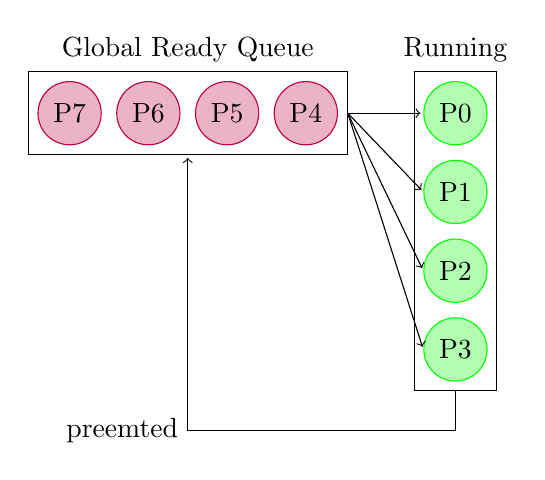
\begin{tikzpicture}[shorten >=1pt,node distance=1.0cm,on grid,auto,
    running/.style={circle, draw=green!100, fill=green!30},
    ready/.style={circle, draw=purple!100, fill=purple!30}
    ]

    \node[ready] (p_4) [] {P4};
    \node[ready] (p_5) [left=of p_4] {P5};
    \node[ready] (p_6) [left=of p_5] {P6};
    \node[ready] (p_7) [left=of p_6] {P7};

    \node[state,rectangle] (q_0) [fit={(p_4) (p_5) (p_6) (p_7)}] [label=Global Ready Queue] {};

    \node[running] (r_0) [right=of q_0, xshift=24mm] {P0};
    \node[running] (r_1) [below=of r_0] {P1};
    \node[running] (r_2) [below=of r_1] {P2};
    \node[running] (r_3) [below=of r_2] {P3};

    \node[state,rectangle] (q_1) [fit={(r_0) (r_1) (r_2) (r_3)}] [label=Running] {};

    \draw[->] (q_0.east) -- (r_0.west);
    \draw[->] (q_0.east) -- (r_1.west);
    \draw[->] (q_0.east) -- (r_2.west);
    \draw[->] (q_0.east) -- (r_3.west);


    \draw[->] (q_1.south) |- ++(0,-5mm) -| (q_0.south) node[midway] {preemted};

    % \node[state,rectangle, align=center] (q_r) [] {This is a \\ square}; % Here the nodes and coordinates are defined
    % \node[coordinate] (q_0) [right=of q_r, xshift=3cm]   {};
    % \node[coordinate] (q_1) [left=of q_r, xshift=-3cm, yshift=1mm]   {};
    % \node[coordinate] (q_2) [left=of q_r, xshift=-3cm, yshift=-1mm]   {};
    % \path[->] % path and draw commands connect the nodes and coordinates to each other.
    % (q_r) edge [] node  {This is an arrow} (q_0);   
    % \draw[->] ([yshift=-3mm]q_1) -- ([yshift=-2mm]q_r.west) node[midway,swap] {This is an arrow};
    % \draw[->] ([yshift=3mm]q_2) -- ([yshift=2mm]q_r.west) node[midway] {This is an arrow};
\end{tikzpicture}


\section{Performance Tests}
\label{sec:perfTests}
Various user programs were tested against different variations of the scheduler.  In general the tests were performed on processes tasked with performing a scalar multiply on a data set with a size relative to the L1 cache.  As a baseline, the OS was configured to run on only a single core and a matrix multiplication was performed on a matrix exactly the size of the cache.  For more interesting results, a data set 4x the size of the cache was tested with the global run-queue and the per-core run-queue with evenly distributed CPU affinity.  In these cases each process would work on an independent part of the data set.  

The impact of per-core scheduler with and without pull migration was analyzed with tasks with varying runtime.  Three classes of processes were defined as short, medium and long; each, with 10x the runtime of the previous case.  An even distribution of each type of task and the data set was tested against these schedulers.  Additionally the schedulers were tested against many short runtime processes compared to the few long runtime processes.

Finally, a common pattern; in resource intensive and parallelizable tasks, is to create a smaller subset of OS tasks and pull work off a shared queue.  Otherwise known as a thread pool, the difference between allowing the OS to manage all the tasks compared to semi-manual work queueing was examined.  Work was divided into 64 threads with 16 workers for the pooled case.  Additionally the locality of the data being worked on was constrained to both 4 (sm) and 16 (lg) matrices of a smaller size than the L1 cache.  All tests ran on the per-core scheduler with pull migration.  

% TODO: remove this, breaking other tables for some reason...
\begin{table}[h!]
    \centering
    \caption{Table to test captions and labels}
\end{table}

\begin{table}[h!]
% \begin{center}
    \centering
    \begin{tabular}{ l|rrr }
        & Total & User & Kernel \\
        \hline
        Instrs & 0 & 0 & 0 \\
        Cycles & 0 & 0 & 0 \\
        Access & 0 & 0 & 0 \\
        Refill & 0 & 0 & 0 \\
        Runtime & 0 & 0 & 0 \\
        \hline
    \end{tabular}
    \caption{table caption}        
% \end{center}
\end{table}

\subsection{Linguistic Features}
\label{subsection:linguistic}

Features. 

\subsubsection{Lexical Features}
\label{subsection:lexicalFeatures}

Other features.

\begin{equation}
H(X|Y) = - \sum_{y \in Y} P(y_i) \sum_{x \in X} p(x_i|y_i)\log p(x_i|y_i)
\label{equation:conditionalEntropy1}
\end{equation}


\section{Conclusion and Future Work}
\label{sec:conclusionAndFutureWork}

Conclusions here.

\section*{Acknowledgements} 
We would like to thank.. 

This work is funded by...


% OBLIGATORY: use BIBTEX formatting!
\small{
\bibliographystyle{cys}
\bibliography{biblio}
}
\normalsize


\begin{biography}[foto.JPG]{John Smith} 
is professor ...
\end{biography}

\begin{biography}[foto.JPG]{Juan Perez} 
is researcher...
\end{biography}

\begin{biography}[foto.JPG]{Ivan Petrov} 
is researcher...
\end{biography}


{\vskip 12pt}
\noindent
\footnotesize {Article received on 06/12/2012; accepted on 16/01/2013.}

\end{document}

